\documentclass[fleqn,10pt]{physiome}
% Use option lineno for line numbers
\usepackage[font=small,labelfont=bf,
   justification=justified,
   format=plain]{caption} % 'format=plain' avoids hanging indentation
\usepackage{appendix}
\usepackage{physics}
\usepackage{xcolor}
\usepackage{float}
\usepackage[section]{placeins}
\definecolor{blueheader}{RGB}{58, 110, 143}
\articletype{Original}
%% Choose from Original, Retrospective, Review, Letter
\newcommand{\note}[1]{}
\renewcommand{\note}[1]{{\color{red} \textit{[{#1}]}}}

\title{Reproducibility study of the Fabbri et al. 2017 model of the human sinus node action potential}

\author[1][nima.afshar@auckland.ac.nz]{Nima Afshar}
\author[2]{Alan Fabbri}
\author[2]{Stefano Severi}
\author[1]{Alan Garny}
\author[1]{David Nickerson}
\affil[1]{Auckland Bioengineering Institute, University of Auckland, New Zealand}
\affil[2]{Computational Physiopathology Unit, Department of Electrical, Electronic and Information Engineering “Guglielmo Marconi”, University of Bologna, Cesena, Italy}

%% The following lines can be omitted when submitting;
%% information will be added by editors
\publicationdate{01 Sept 2021}
\editor{Shelley Fong}
\curator{Weiwei Ai}
\submitteddate{11 Aug 2021}
\accepteddate{01 Sept 2021}
\citethisas{Afshar and Fabbri. Reproducibility study of the Fabbri et al. 2017 model of the human sinus node action potential. \\ Physiome.}{10.36903/physiome.16550526}
\begin{document}

\maketitle

\begin{abstract}
The sinoatrial node (SAN) is the natural pacemaker of the mammalian heart. It has been the subject of several mathematical studies, aimed at reproducing its electrical response under normal sinus rhythms, as well as under various conditions.

Such studies were traditionally done using data from rabbit SAN cells. More recently, human SAN cell data have become available, resulting in the publication of a human SAN cell model \citep{fabbri2017computational}, along with its CellML version.

Here, we used the CellML file provided by the model authors, together with some SED-ML files and Python scripts that we created to reproduce the main results of the aforementioned modelling study.
\end{abstract}

\keywords{Physiome, CellML, OpenCOR, reproducibility, action potentials, cardiac electrophysiology, cardiovascular models, ion channels, sinoatrial node}

\primarypubs[10.36903/physiome.16550526]{main}{fabbri2017computational}

\section{Introduction}

The sinoatrial node (SAN) plays an important role in cardiac function and although it has been extensively studied, some of its intrinsic mechanisms are still open for debate. Most of the experimental data used in SAN modelling have been carried out on animals and on rabbits in particular \citep{lakatta2009keeps, difrancesco2010role, lakatta2010paradigm, maltsev2010funny, noble2010competing, verkerk2007pacemaker, himeno2008ionic, difrancesco2012funny, lakatta2012rebuttal, rosen2012case, monfredi2013modern, yaniv2013new, yaniv2015two}. This has resulted in the development of comprehensive SAN models \citep{wilders2007computer}. Yet, this body of work can hardly be transposed to humans.

Human SAN action potentials were first recorded by \citet{drouin1997electrophysiologic}, followed by \citeauthor{verkerk2007pacemaker} a decade later \citep{verkerk2007pacemaker, verkerk2013calcium}. The first human SAN cell model was developed as a proof-of-concept by \citet{seemann2006heterogeneous}. This was followed by the model of \citet{chandler2009molecular}. More recently, \citet{verkerk2015pacemaker} studied the effect of mutations on human SAN cells, highlighting the need for a human-specific SAN cellular electrophysiology model. Such a model was formulated by \citet{pohl2016computational}, but its action potential shape does not match that of experimental recordings. \citet{fabbri2017computational} addressed this shortcoming by developing their human SAN cell model using available human electrophysiological data.

\citet{fabbri2017computational} published a CellML version \citep{cuellar2003overview} of their model on the Physiome Model Repository \citep{yu_physiome_2011}. However, the CellML file on its own is not sufficient to reproduce all predictions presented in the primary paper. Some SED-ML files \citep{waltemath2011reproducible} and Python scripts were therefore created and used with the aforementioned CellML file to reproduce the main results from \citet{fabbri2017computational}. No modifications were made to the CellML file mathematics or parameters and all the equations and parameters can be found in the original paper.

\section{Model description}

\citet{fabbri2017computational} developed a human SAN cell model, based on the rabbit SAN cell model of \citet{severi2012updated} and on recent electrophysiological data from human SAN cells. The resulting action potential and calcium transient are in agreement with experimentally recorded values. Mutations associated with sinus node dysfunction were also modelled and their effects on pacing rate agree with clinical observations.

The model was developed in Simulink and simulations performed using MATLAB's ode15s solver \citep{shampine1997matlab}. Simulations were run until calcium dynamics reached steady‐state. Custom MATLAB (2013a) code was used for automatic optimization and feature extraction. A CellML-encoded version of the model is available at \url{https://models.physiomeproject.org/e/568}.

The simulation results presented here were produced using the 2021-07-09 snapshot of OpenCOR \citep{garny2015opencor} together with various Python scripts that rely on a SED-ML file to configure (the solver to use, the duration of the simulation, the model parameters to track, etc.) and run a given simulation using the model encoded in CellML. Python scripts are also used to generate the figures using Matplotlib \citep{Hunter:2007}.

\section{Model results}

\begin{figure}[htb]
\centering
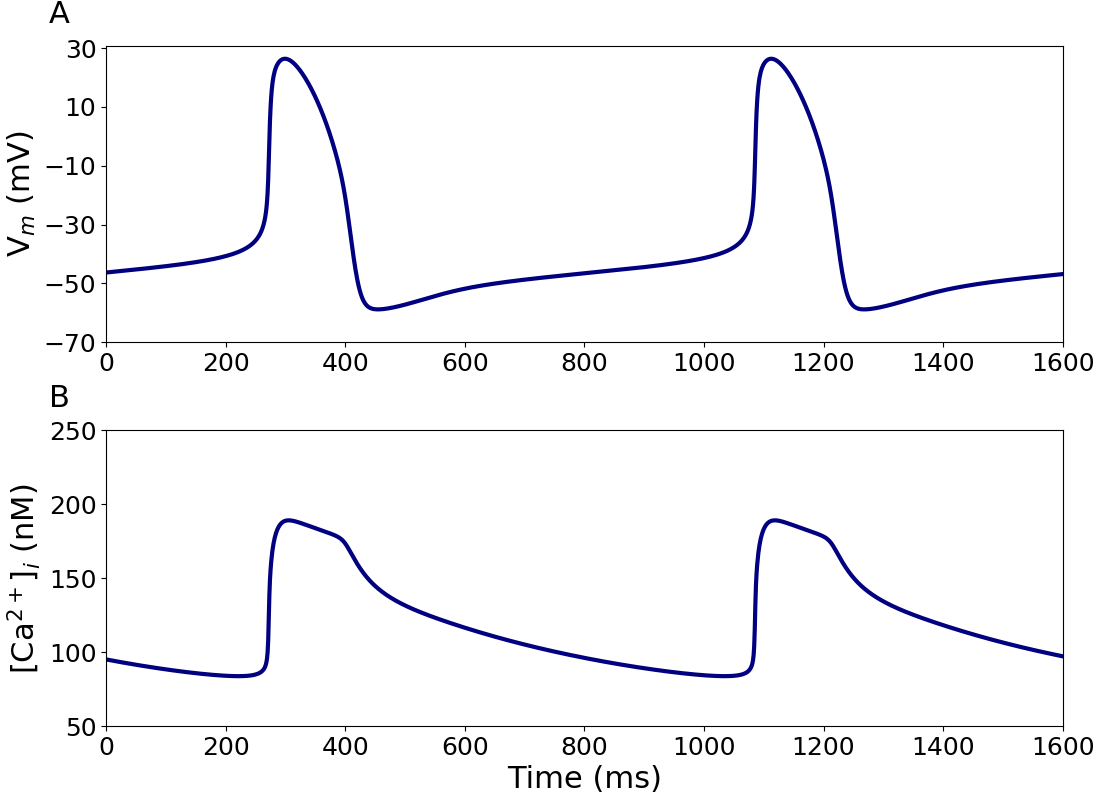
\includegraphics[width=0.7\linewidth]{Figure1}
\caption{\textbf{Action potential and intracellular calcium transient of a single human SAN cell.}\newline
Simulated action potential (AP; A) and associated calcium transient (\textit{[Ca\textsuperscript{2+}]\textsubscript{i}}; B) of a single human SAN cell. This figure can be reproduced using \href{https://models.physiomeproject.org/workspace/648/rawfile/6784d6c3256c832dc98b2db42c85747ae2596518/Figure1.py}{Figure1.py}.}
\label{Figure1}
\end{figure}

\autoref{Figure1} shows the action potential (A) and intracellular calcium transient (B), as computed by the model. It reproduces Figure~2 of the primary paper with a cycle length of 814 ms which corresponds to a beating rate of 74 beats min\textsuperscript{-1}. In \autoref{Figure2}, the time course of the simulated action potential (A) and its underlying components (B-K) are shown, which corresponds to Figure 3 in the primary paper.

\begin{figure}[htb]
\centering
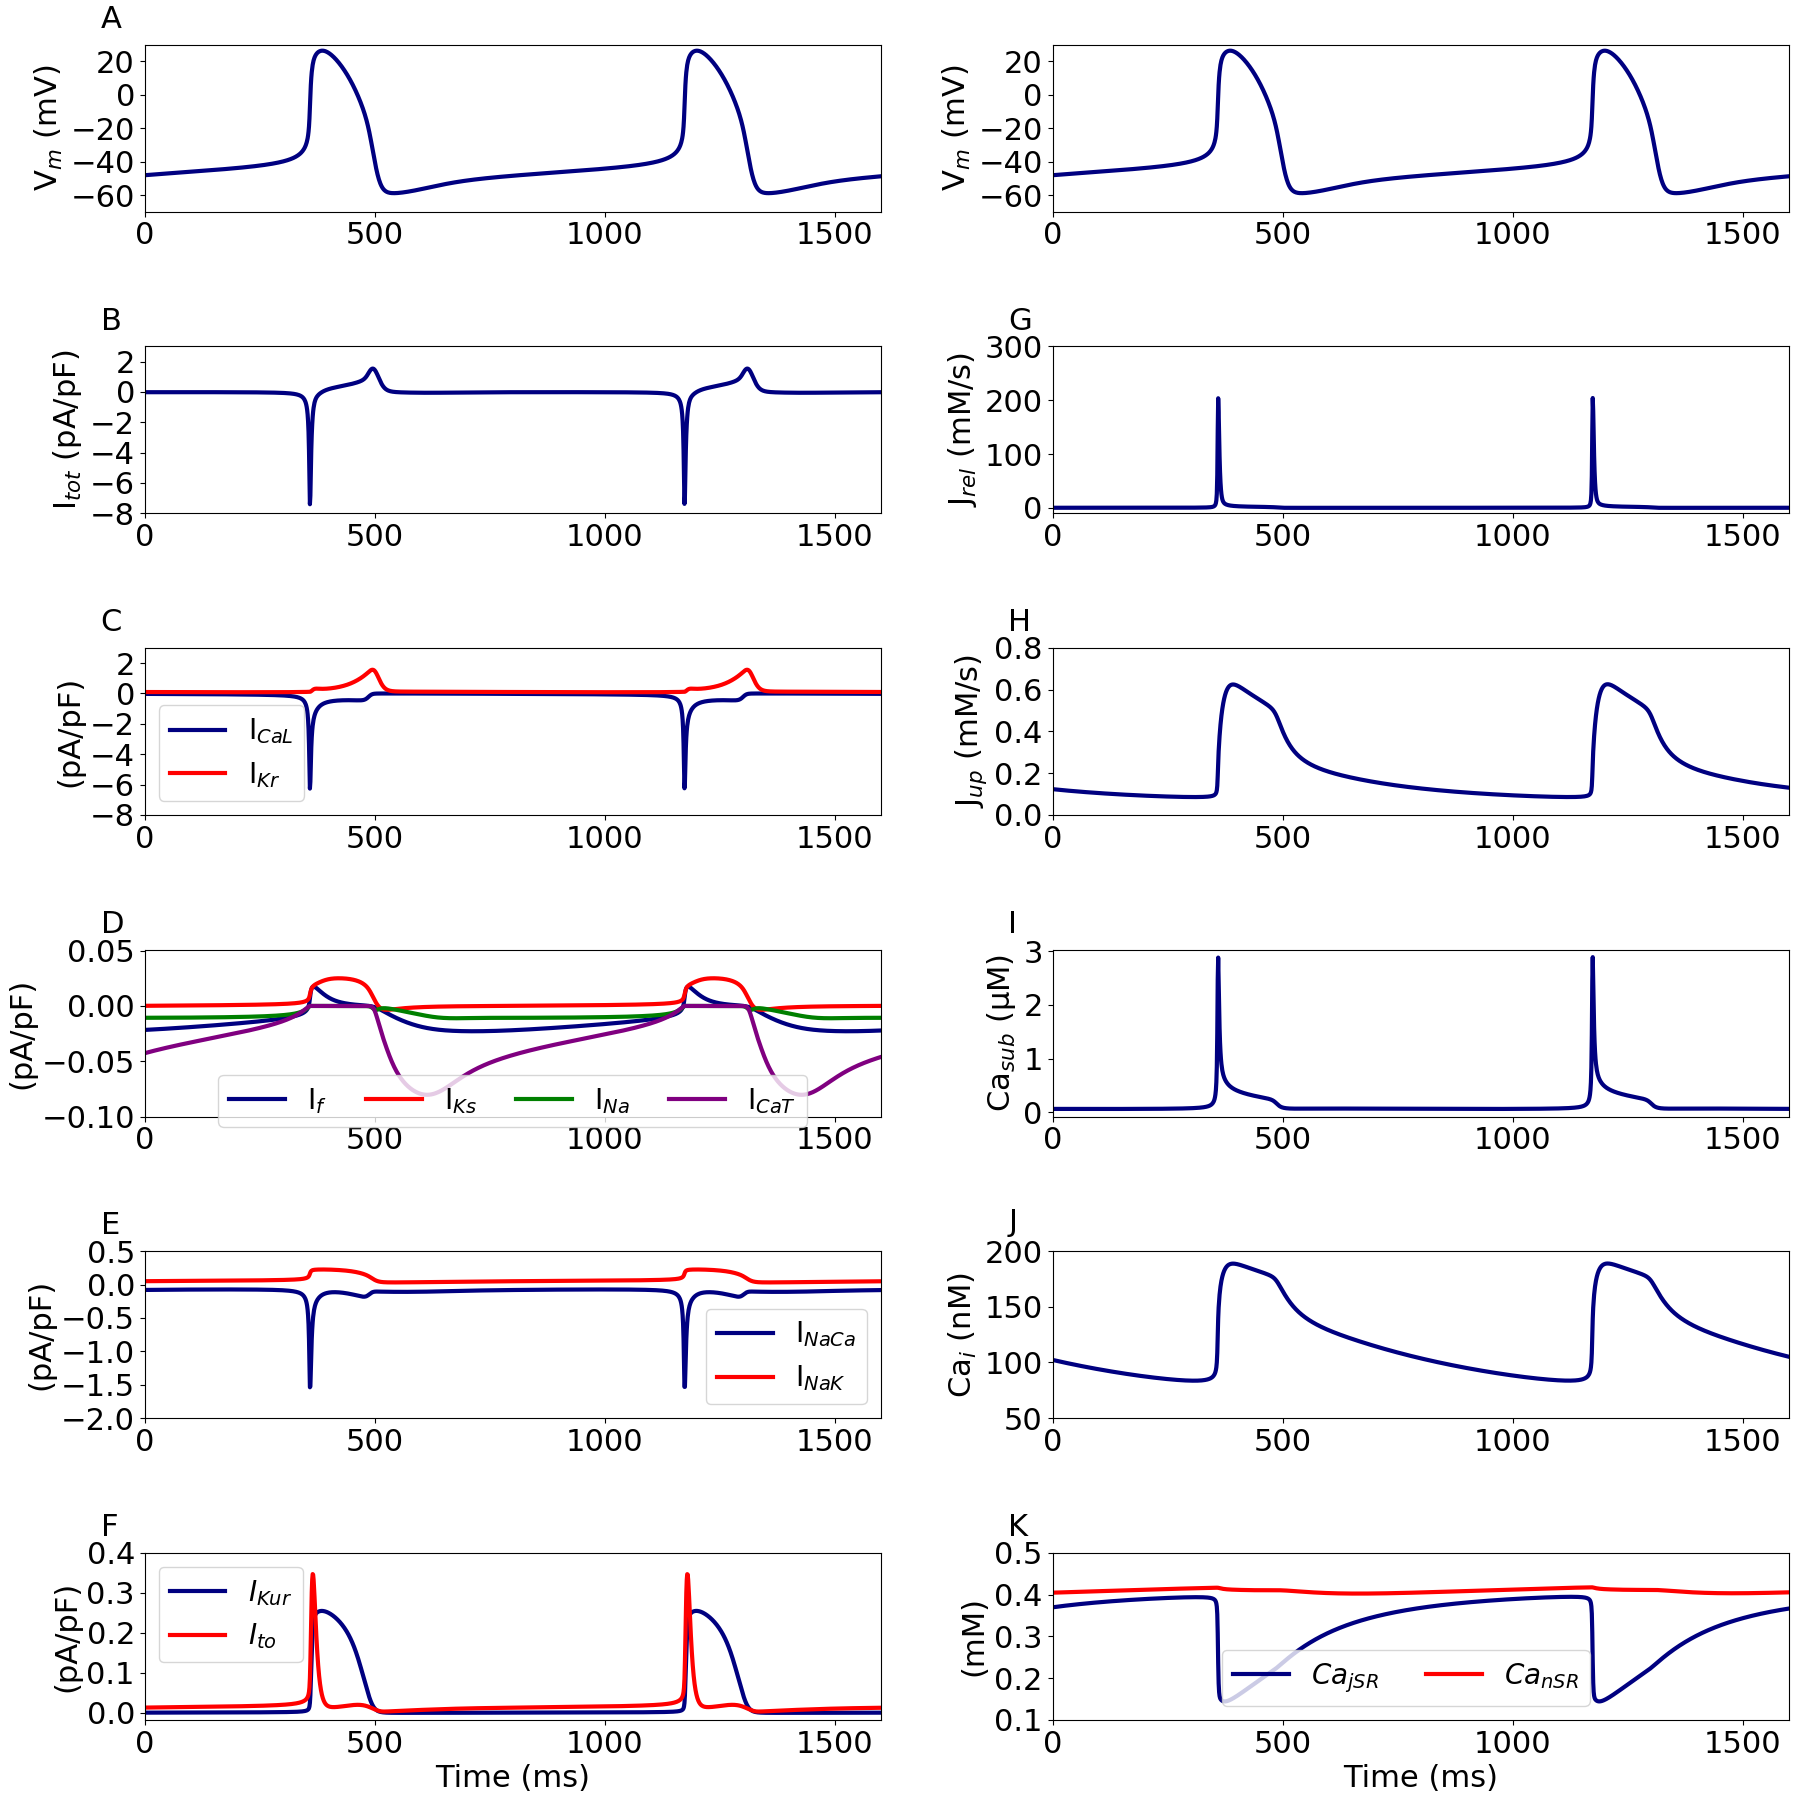
\includegraphics[width=1\linewidth]{Figure2}
\caption{\textbf{Time course of the simulated action potential and its underlying ionic currents.}\newline
Simulated AP (A) and associated currents (B-F), fluxes (G \& H), and calcium concentrations (I-K). The top right panel is a copy of panel A and is included for convenience and to match Figure 3 in the primary paper. This figure can be reproduced using \href{https://models.physiomeproject.org/workspace/648/rawfile/6784d6c3256c832dc98b2db42c85747ae2596518/Figure2.py}{Figure2.py}.}
\label{Figure2}
\end{figure}

\autoref{Figure3} shows the membrane potential and its associated currents during diastolic depolarization. The resulting behaviour corresponds to that presented in Figure~4 in the primary paper.

\begin{figure}[htb]
\centering
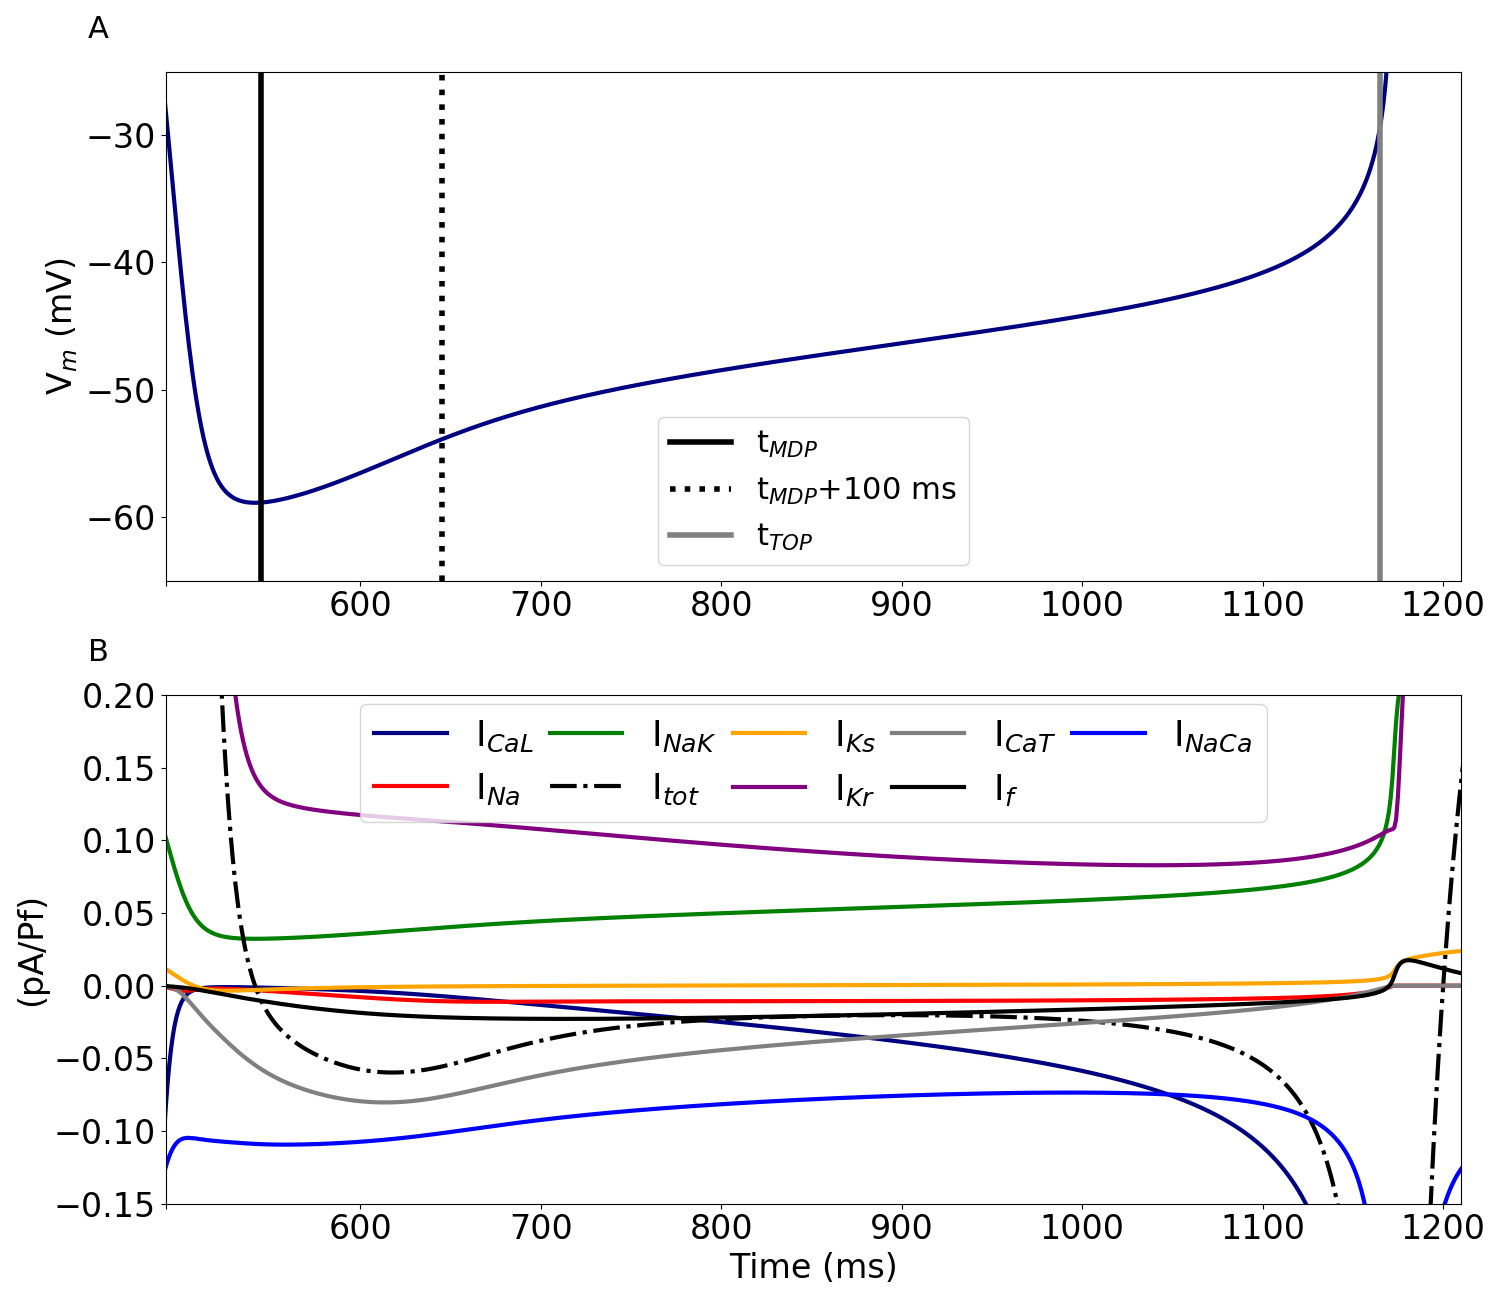
\includegraphics[width=0.8\linewidth]{Figure3}\newline
\caption{\textbf{Membrane currents underlying diastolic depolarization.}\newline
Simulated AP (A) and associated membrane currents (B). t\textsubscript{MDP} and t\textsubscript{TOP} indicate the time at which the membrane potential (V\textsubscript{m}) is at its maximum diastolic potential (MDP) and take-off potential, respectively. This figure can be reproduced using \href{https://models.physiomeproject.org/workspace/648/rawfile/6784d6c3256c832dc98b2db42c85747ae2596518/Figure3.py}{Figure3.py}.}
\label{Figure3}
\end{figure}

\begin{figure}[htb!]
\centering
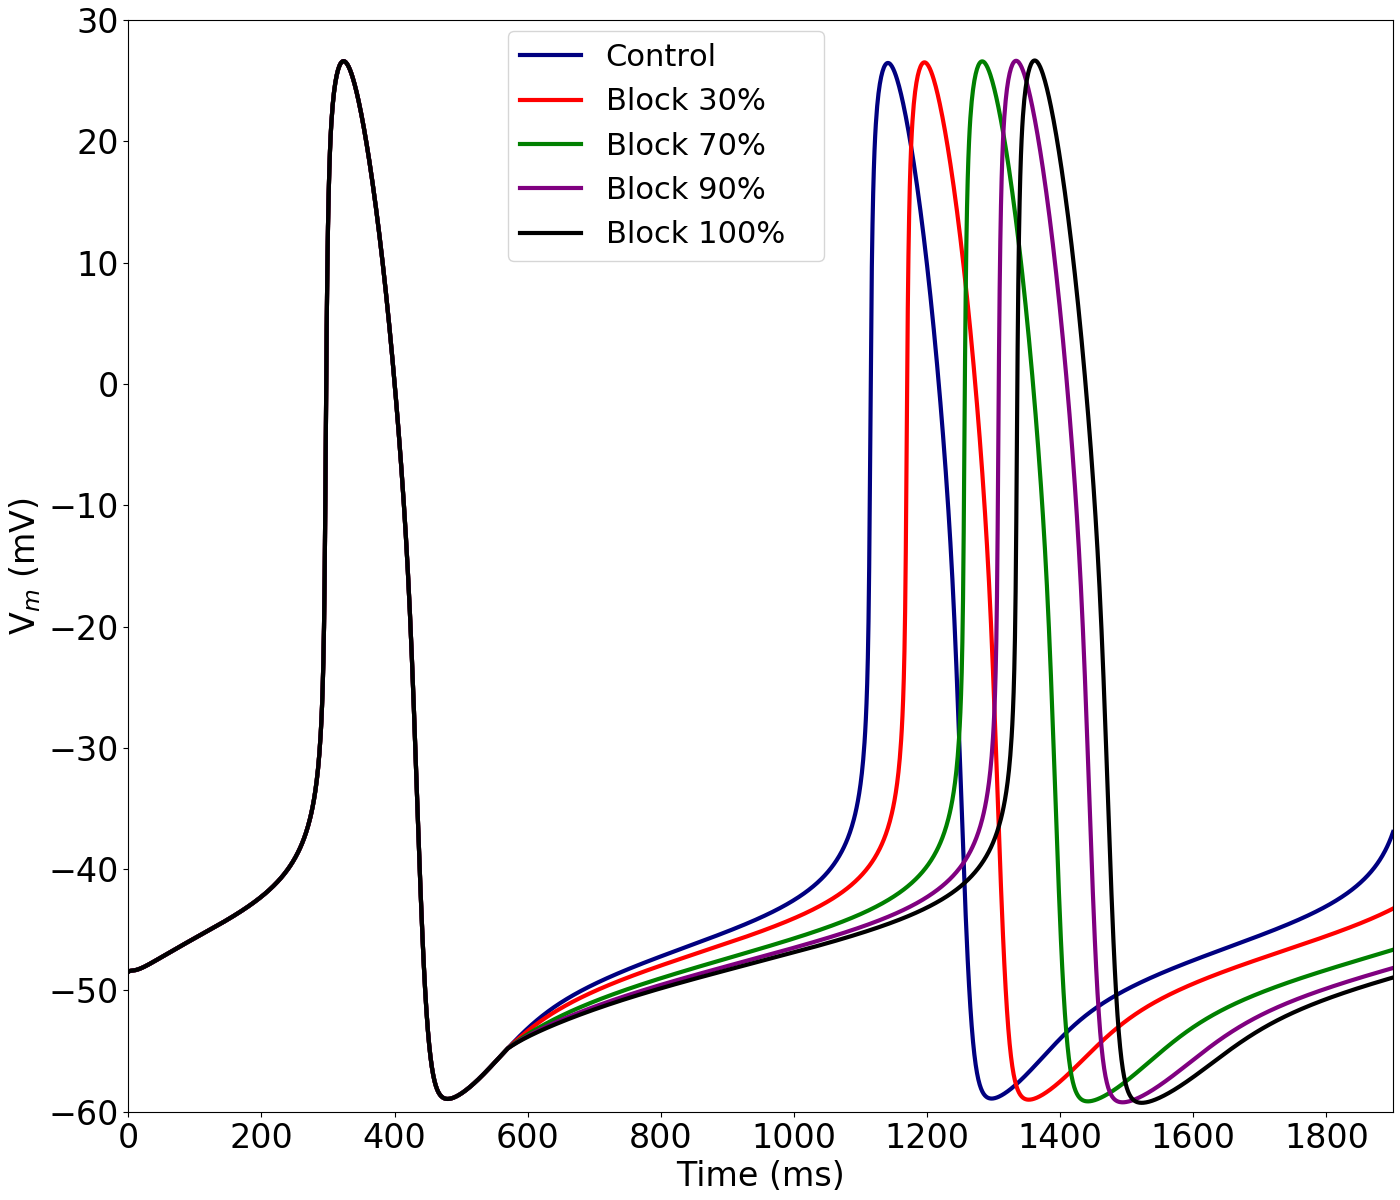
\includegraphics[width=0.7\linewidth]{Figure4}
\caption{\textbf{Functional effect of $I_{f}$ block.}\newline
Simulated AP under control conditions (CTRL) and upon 30\%, 70\%, 90\% and full block of the funny current (\textit{I\textsubscript{f}}). This figure can be reproduced using \href{https://models.physiomeproject.org/workspace/648/rawfile/6784d6c3256c832dc98b2db42c85747ae2596518/Figure4.py}{Figure4.py}.}
\label{Figure4}
\end{figure}

In \autoref{Figure4}, the model is used to reproduce the results of a progressive block of the funny current, \textit{I\textsubscript{f}}, to show its effect on the cycle length (CL) and, therefore, on the pacing rate. This corresponds to Figure~7 in the primary paper.\newpage



\autoref{Figure5} shows the effect of a shift in the activation curve of \textit{I\textsubscript{f}} on the CL (A), the diastolic depolarization rate over the first 100 ms of diastolic depolarization (DDR\textsubscript{100}; B), the maximum diastolic potential (MDP; C), and the action potential duration at 90\% repolarization (APD\textsubscript{90}; D). This corresponds to Figure~8 in the primary paper. As reported in \citet{fabbri2017computational}, little variation in APD\textsubscript{90} is observed, albeit with slight differences between the Python implementation presented here and the original MATLAB implementation used in the primary paper.

\begin{figure}[htb]
\centering
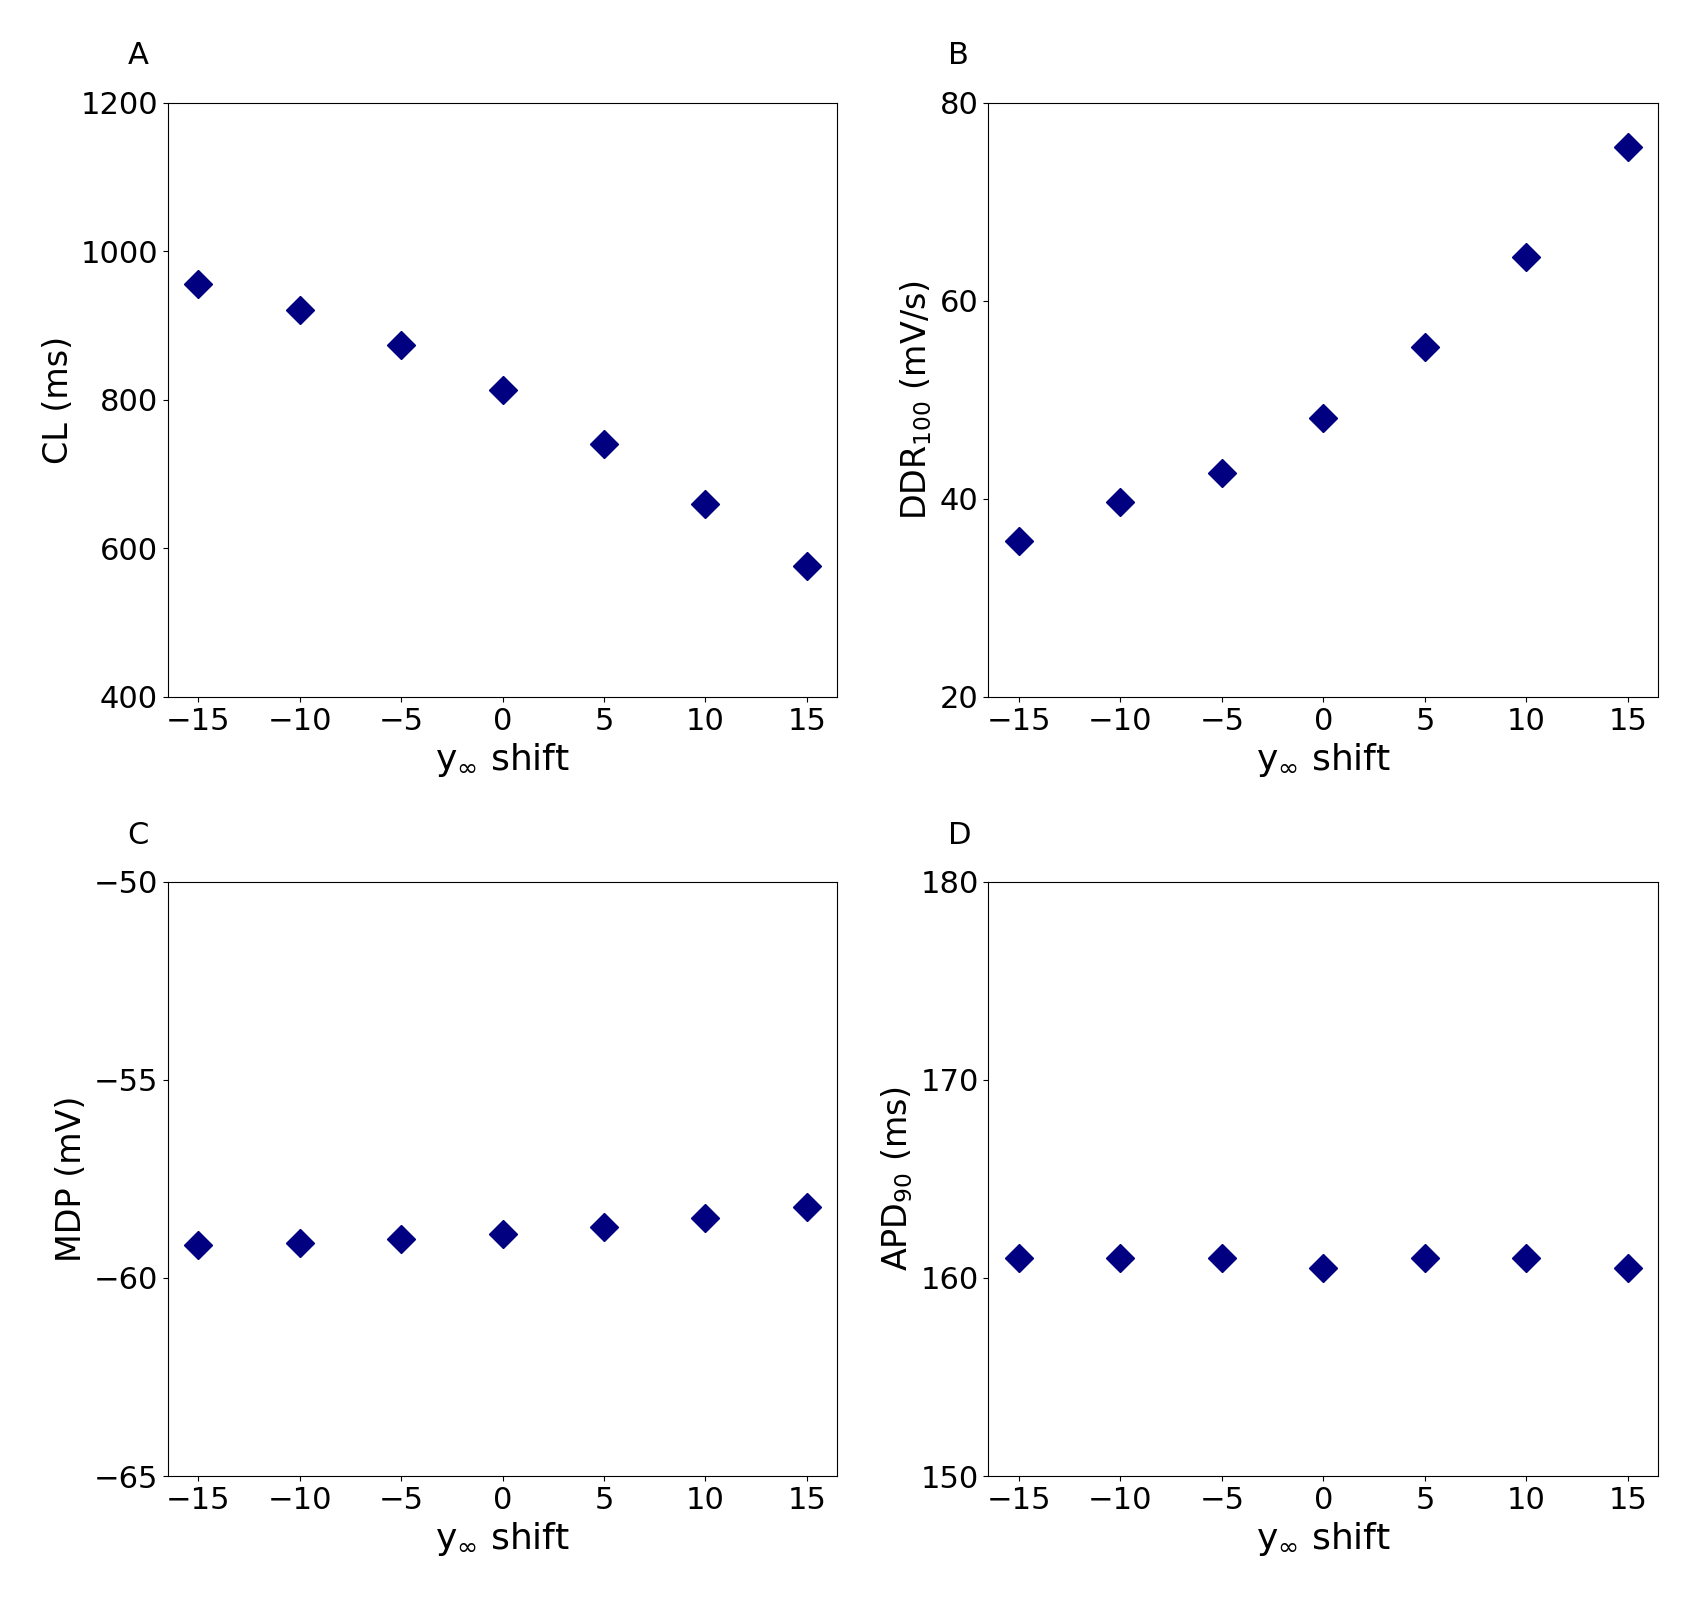
\includegraphics[width=0.9\linewidth]{Figure5}
\caption{\textbf{Functional effect of changes in the voltage dependence of $I_{f}$ activation.}\newline
Simulations of the effect of –15 to +15 mV shifts in the voltage dependence of the steady‐state activation curve (y\textsubscript{$\infty$}) of \textit{I\textsubscript{f}} on the cycle length (CL; A), diastolic depolarization rate over the first 100 ms of diastolic depolarization (DDR\textsubscript{100}; B), MDP (C), and action potential duration at 90\% repolarization (APD\textsubscript{90}; D). This figure can be reproduced using \href{https://models.physiomeproject.org/workspace/648/rawfile/6784d6c3256c832dc98b2db42c85747ae2596518/Figure5.py}{Figure5.py}.}
\label{Figure5}
\end{figure}

The contribution of the sodium-calcium exchanger, \textit{I\textsubscript{NaCa}}, to the action potential is illustrated in \autoref{Figure6}, where a progressive block of \textit{I\textsubscript{NaCa}} was performed. This corresponds to Figure~9 in the primary paper, although the results are slightly different.\newpage

\begin{figure}[htbp]
\centering
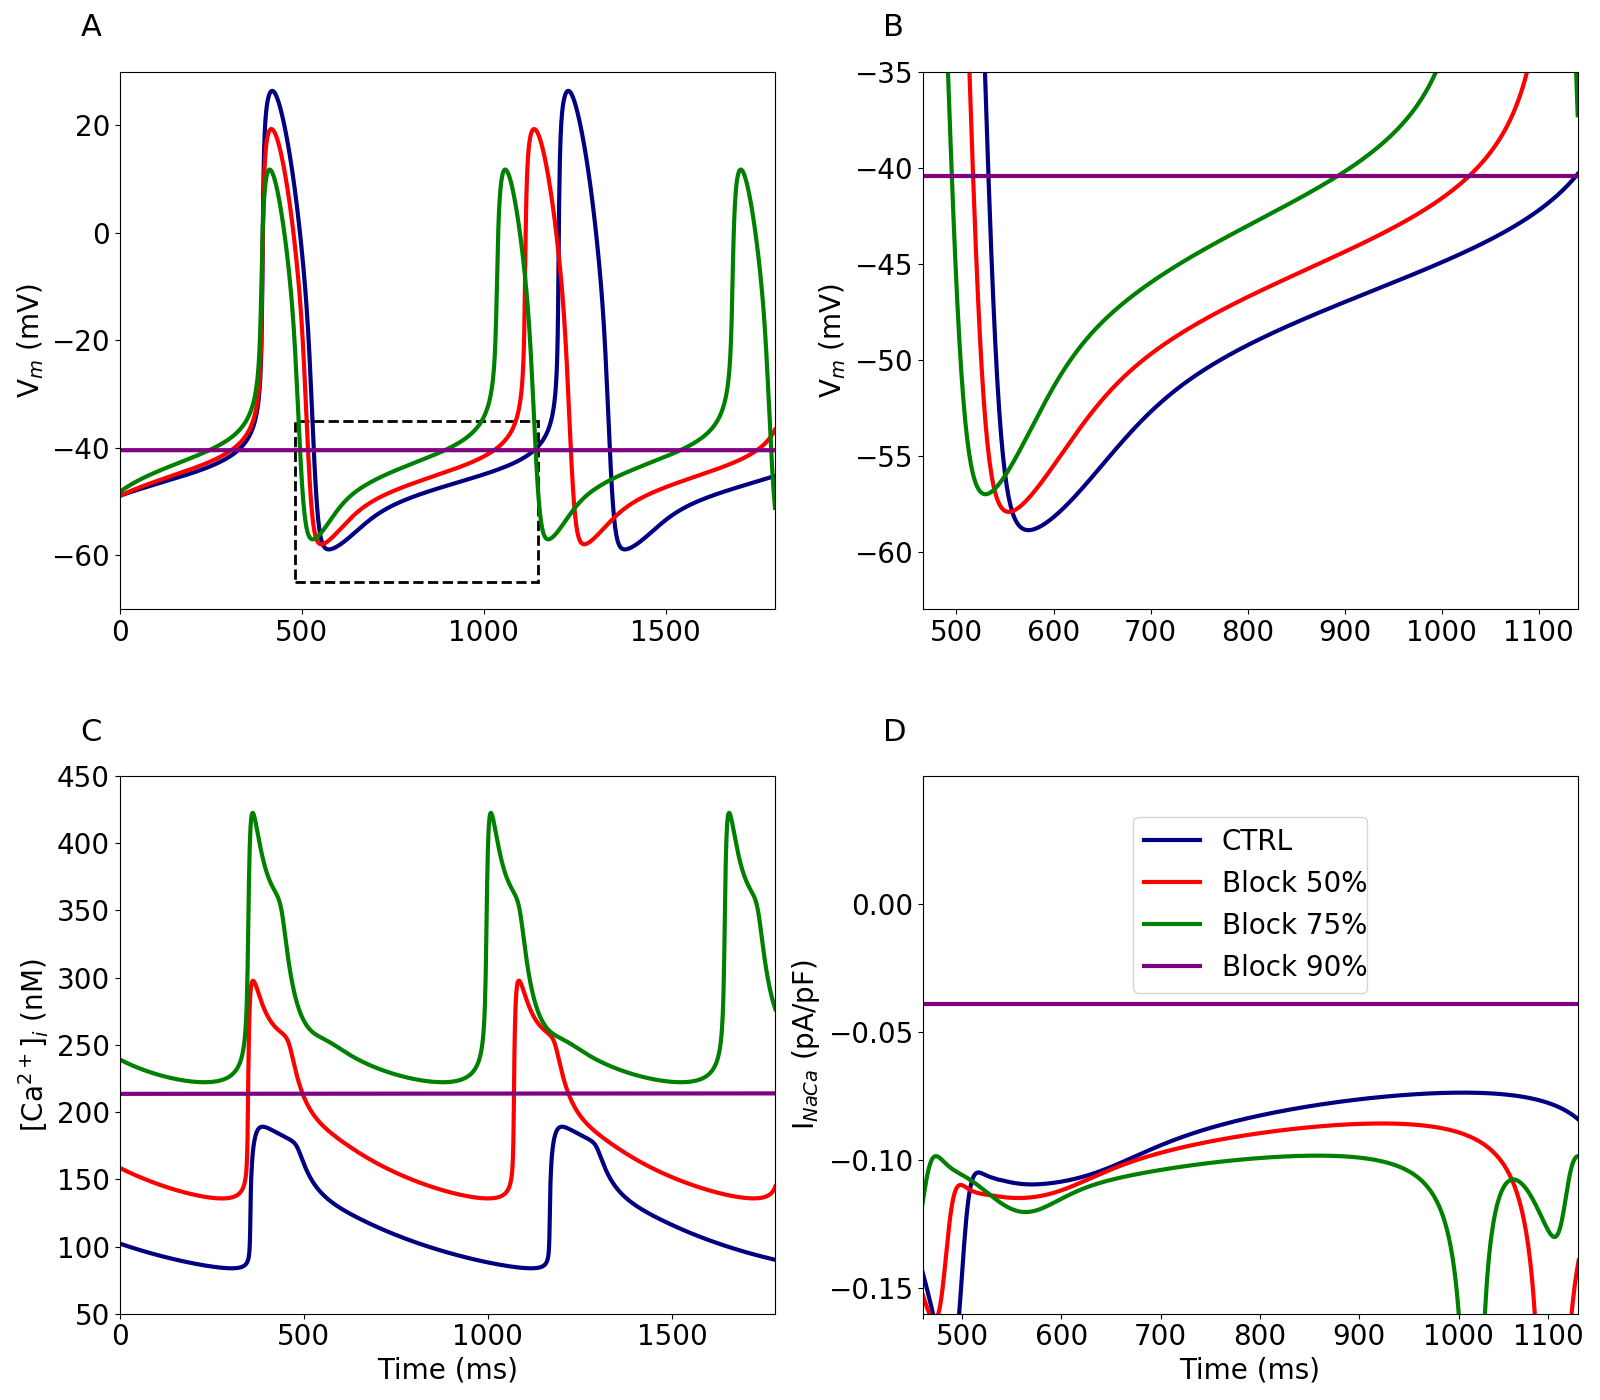
\includegraphics[width=0.95\linewidth]{Figure6}
\caption{\textbf{Functional effect of $I_{NaCa}$ block.}\newline
Time course of the simulated AP (A) and associated [Ca\textsuperscript{2+}]\textsubscript{i} (C) under control conditions (CTRL) and upon 50\%, 75\% and 90\% block of \textit{I\textsubscript{NaCa}}. Time course of the simulated AP (B) and associated \textit{I\textsubscript{NaCa}} (D) relative to the dashed box of (A). This figure can be reproduced using \href{https://models.physiomeproject.org/workspace/648/rawfile/6784d6c3256c832dc98b2db42c85747ae2596518/Figure6.py}{Figure6.py}.}
\label{Figure6}
\end{figure}

\autoref{Figure7} shows the effect of acetylcholine (ACh) and isoprenaline (Iso) on the membrane potential, its net current, the respective target currents for ACh and Iso, and on the sarco‐endoplasmic reticulum Ca\textsuperscript{2+}‐ATPase (SERCA) pump uptake rate. This corresponds to Figure~10 in the primary paper.
\begin{figure}[htbp]
\centering
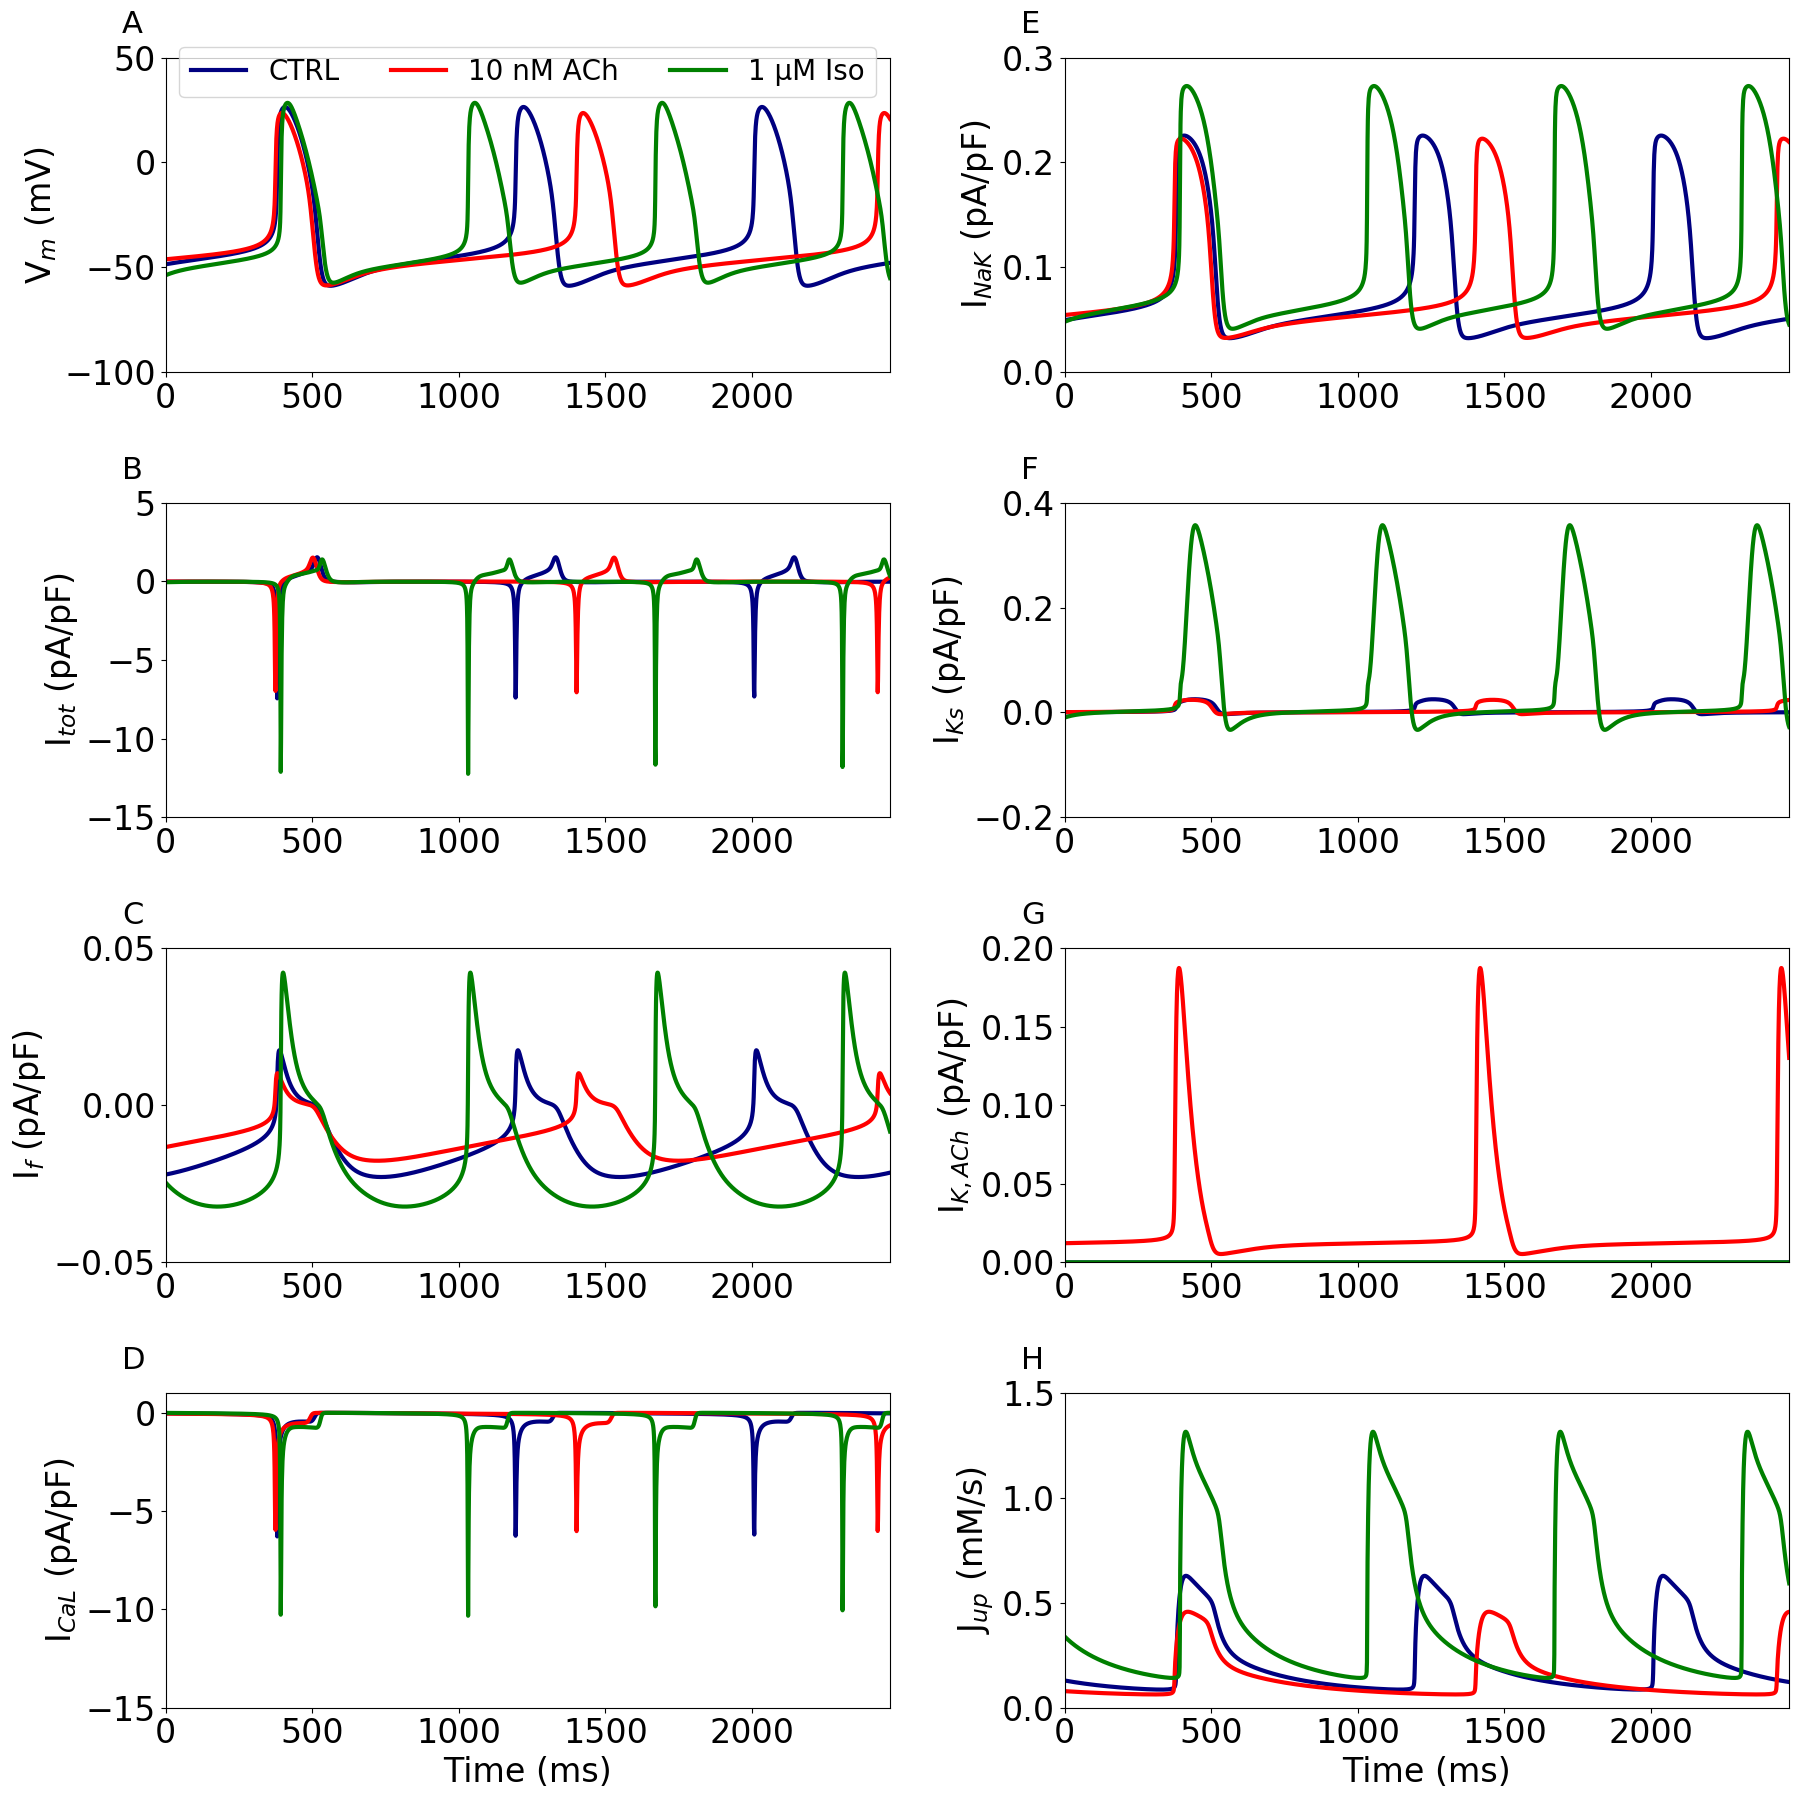
\includegraphics[width=0.95\linewidth]{Figure7}
\caption{\textbf{Functional effect of acetylcholine and isoprenaline.}\newline
Time course of the membrane potential (A), net current (B), target currents (C–G), and SERCA‐pump uptake rate (H) under control conditions (CTRL) and upon administration of 10 nM acetylcholine (ACh) and 1 $\mu$M isoprenaline (Iso). The targets for ACh are \textit{I\textsubscript{f}}, \textit{I\textsubscript{CaL}}, \textit{I\textsubscript{K,ACh}} and \textit{J\textsubscript{up}} while \textit{I\textsubscript{f}}, \textit{I\textsubscript{CaL}}, \textit{I\textsubscript{NaK}}, \textit{I\textsubscript{Ks}} and \textit{J\textsubscript{up}} for Iso. Note the differences in ordinate scales. This figure can be reproduced using \href{https://models.physiomeproject.org/workspace/648/rawfile/6784d6c3256c832dc98b2db42c85747ae2596518/Figure7.py}{Figure7.py}.}
\label{Figure7}
\end{figure}

\section{Discussion}

In this manuscript, we used the CellML version of the human SAN cell model that was developed by \citet{fabbri2017computational}. Most of the main figures in the primary paper were reproducible using the provided CellML code. In some cases, some Python code was needed and can be found at \url{https://models.physiomeproject.org/workspace/648}.\newline

\bibliography{main}

\end{document}